\documentclass[svgnames,11pt]{beamer}
\setbeamercolor{structure}{fg=SlateGray}
\usetheme{Goettingen}
\input{/home/tof/Documents/Cozy/latex-include/preambule_commun.tex}
\usepackage{pgfpages}
\setbeameroption{show notes on second screen=left}
\author[]{Christophe Viroulaud}
\title{Applications Android}
\date{}
%\logo{}
%\institute{Seconde SNT}
\institute{Première NSI}
%\institute{Terminale NSI}
\setbeamertemplate{navigation symbols}{}
\setbeamertemplate{footline}[frame number]

\begin{document}
\begin{frame}
    \titlepage
    \note{\fcolorbox{black}{red}{{\LARGE mettre googleplaystore.zip sur site}}

        googleplaystore.csv, specifications-app.csv, notes.csv}
\end{frame}

\section{Problématique}
\begin{frame}
    \frametitle{Un moteur de recherche pour aider l'utilisateur à faire son choix.}
    \begin{center}
        \centering
        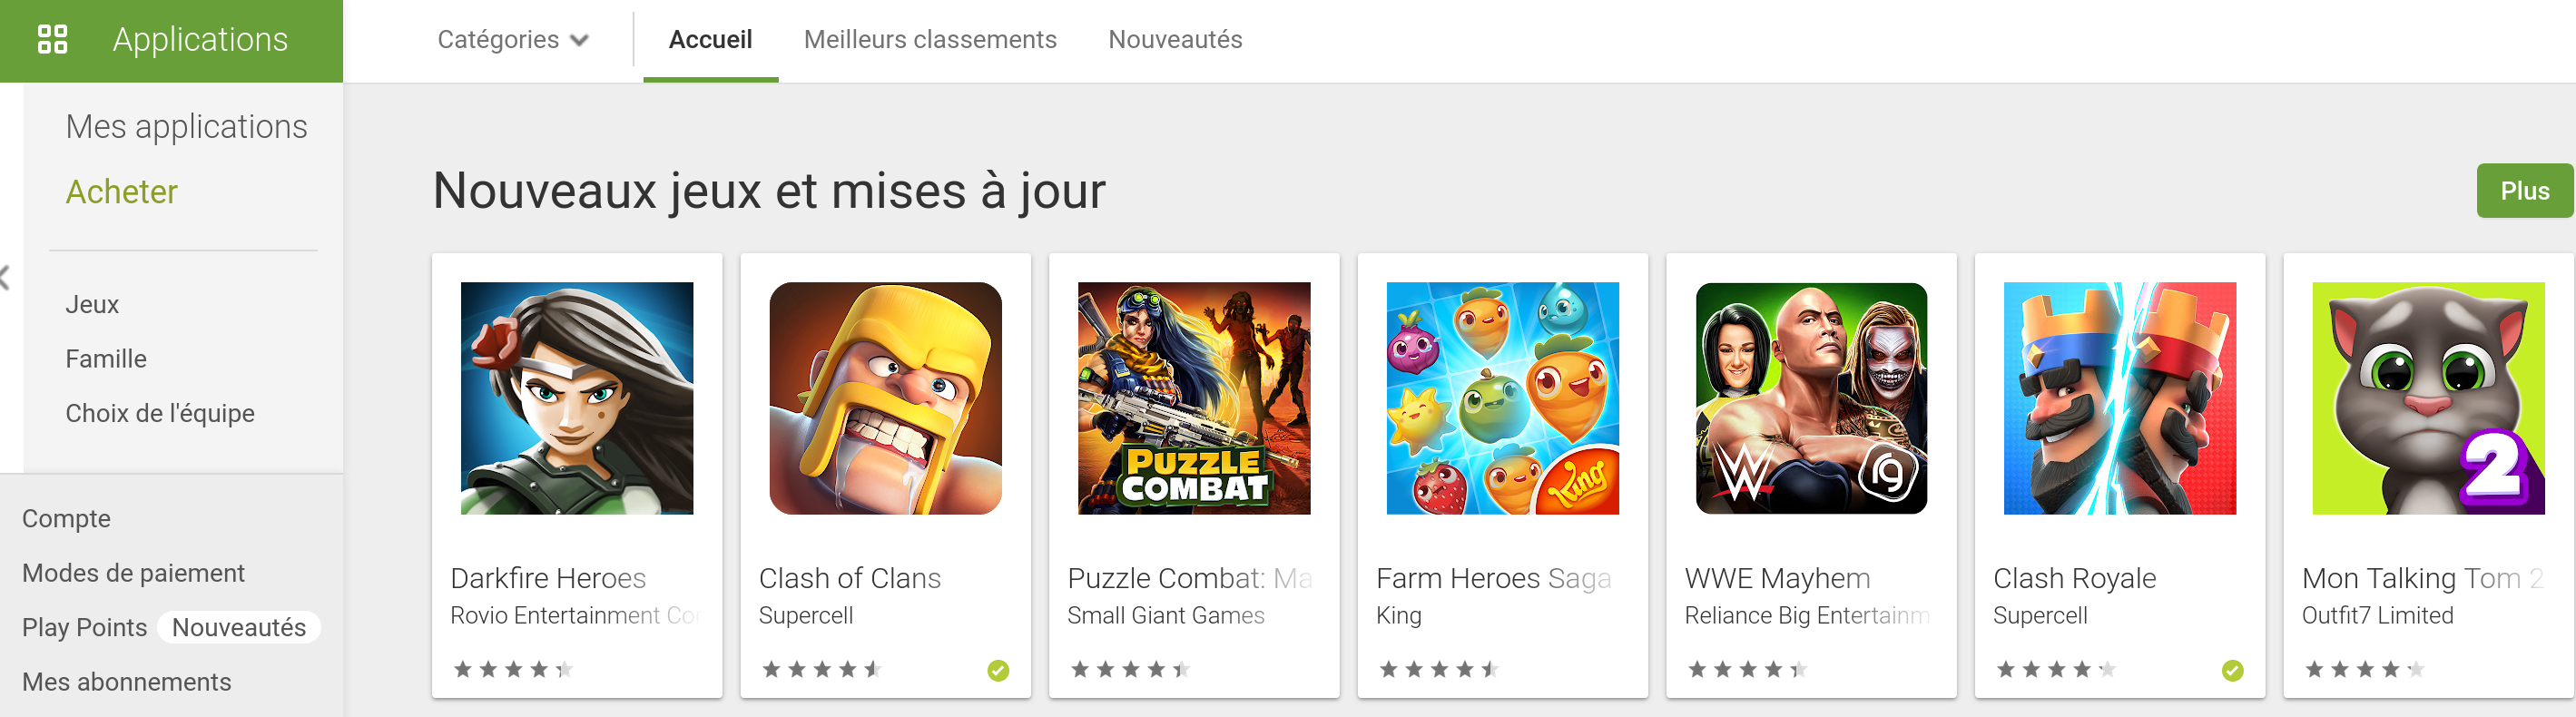
\includegraphics[width=8cm]{ressources/playstore.png}
        \captionof{figure}{Magasin d'applications}
        \label{IMG}
    \end{center}

\end{frame}

\begin{frame}
    \frametitle{Jeu de données}
    \begin{center}
        \centering
        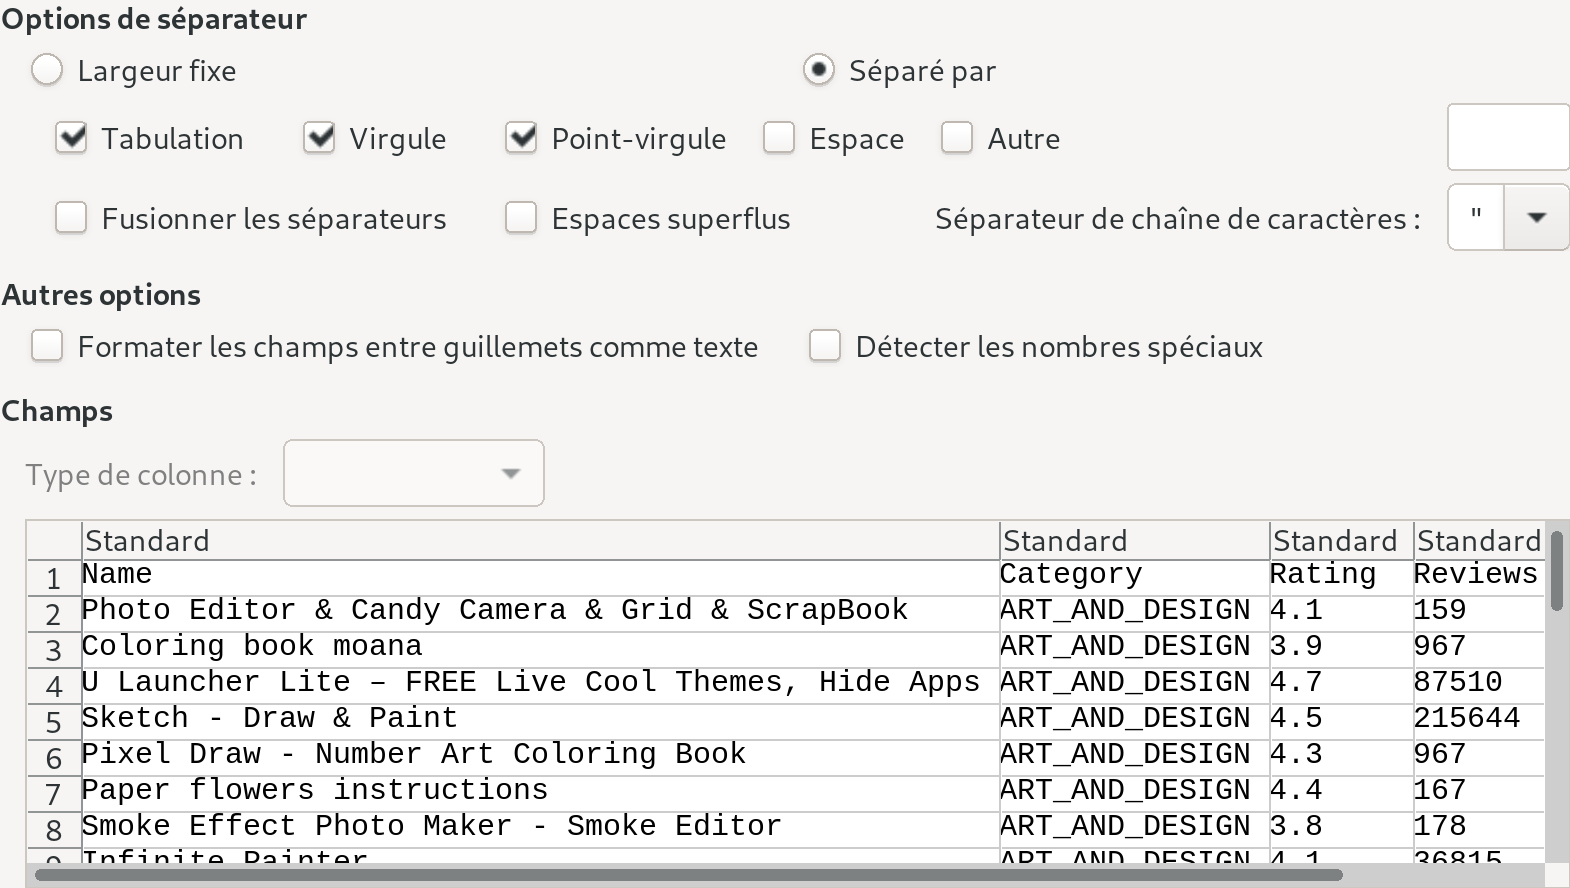
\includegraphics[width=8cm]{ressources/jeu-donnees.png}
        \captionof{figure}{Données dans un fichier texte}
        \label{IMG}
    \end{center}
    \note{dataset}
    \begin{center}
        \framebox{Comment manipuler un jeu de données?}
    \end{center}

\end{frame}
\section{Données en table}
\subsection{Présentation}
\begin{frame}
    \frametitle{Vocabulaire des bases de données}

    \note{terme BDD: entité, table (ou relation), attributs}
    \begin{center}
        \centering
        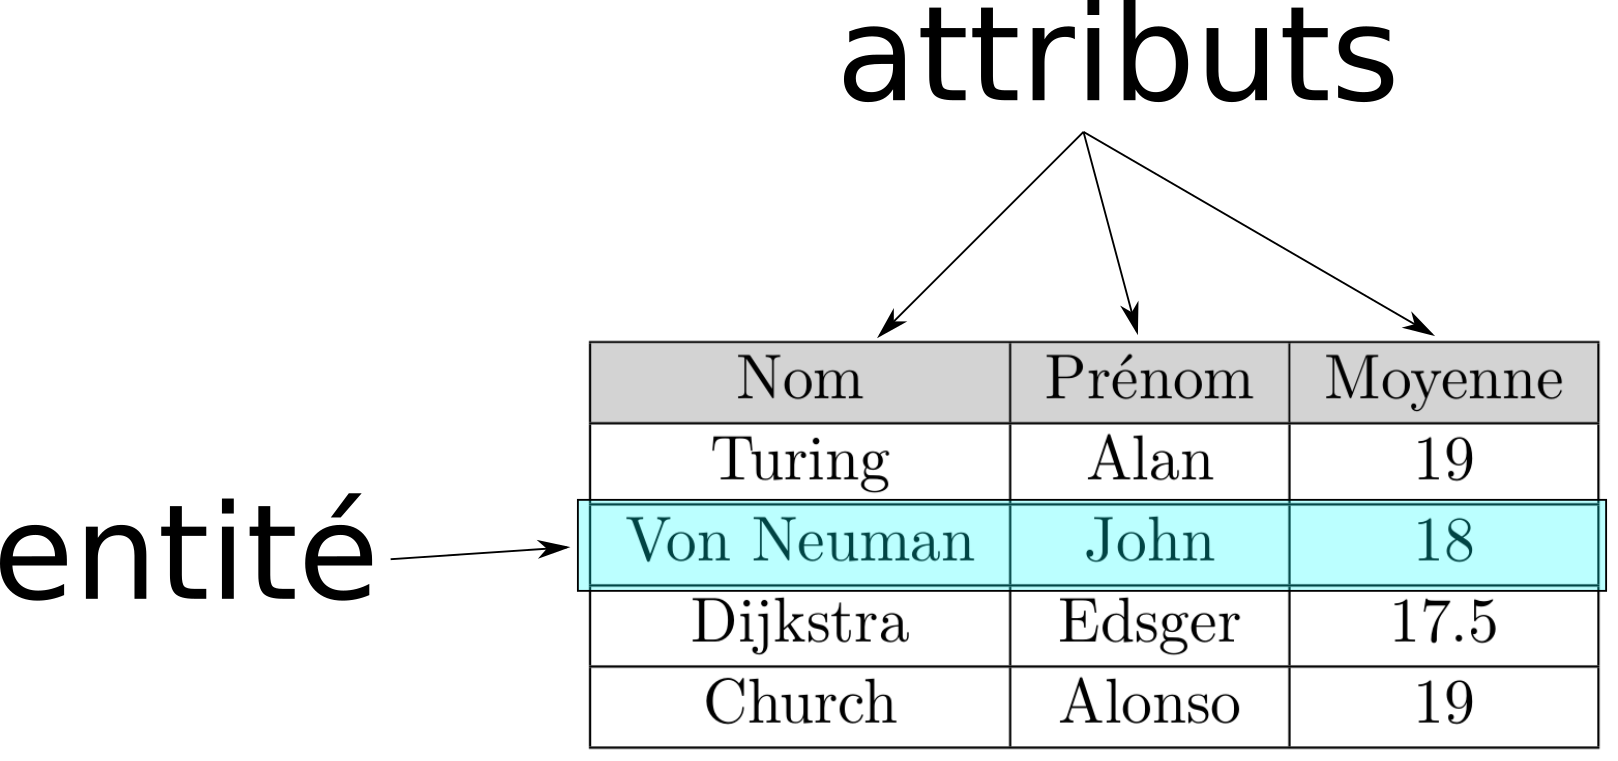
\includegraphics[width=8cm]{ressources/vocabulaire-legende.png}
        \captionof{figure}{Table de données}
        \label{IMG}
    \end{center}

\end{frame}
\begin{frame}
    \frametitle{csv (Comma Separated Values)}

    \begin{center}
        \centering
        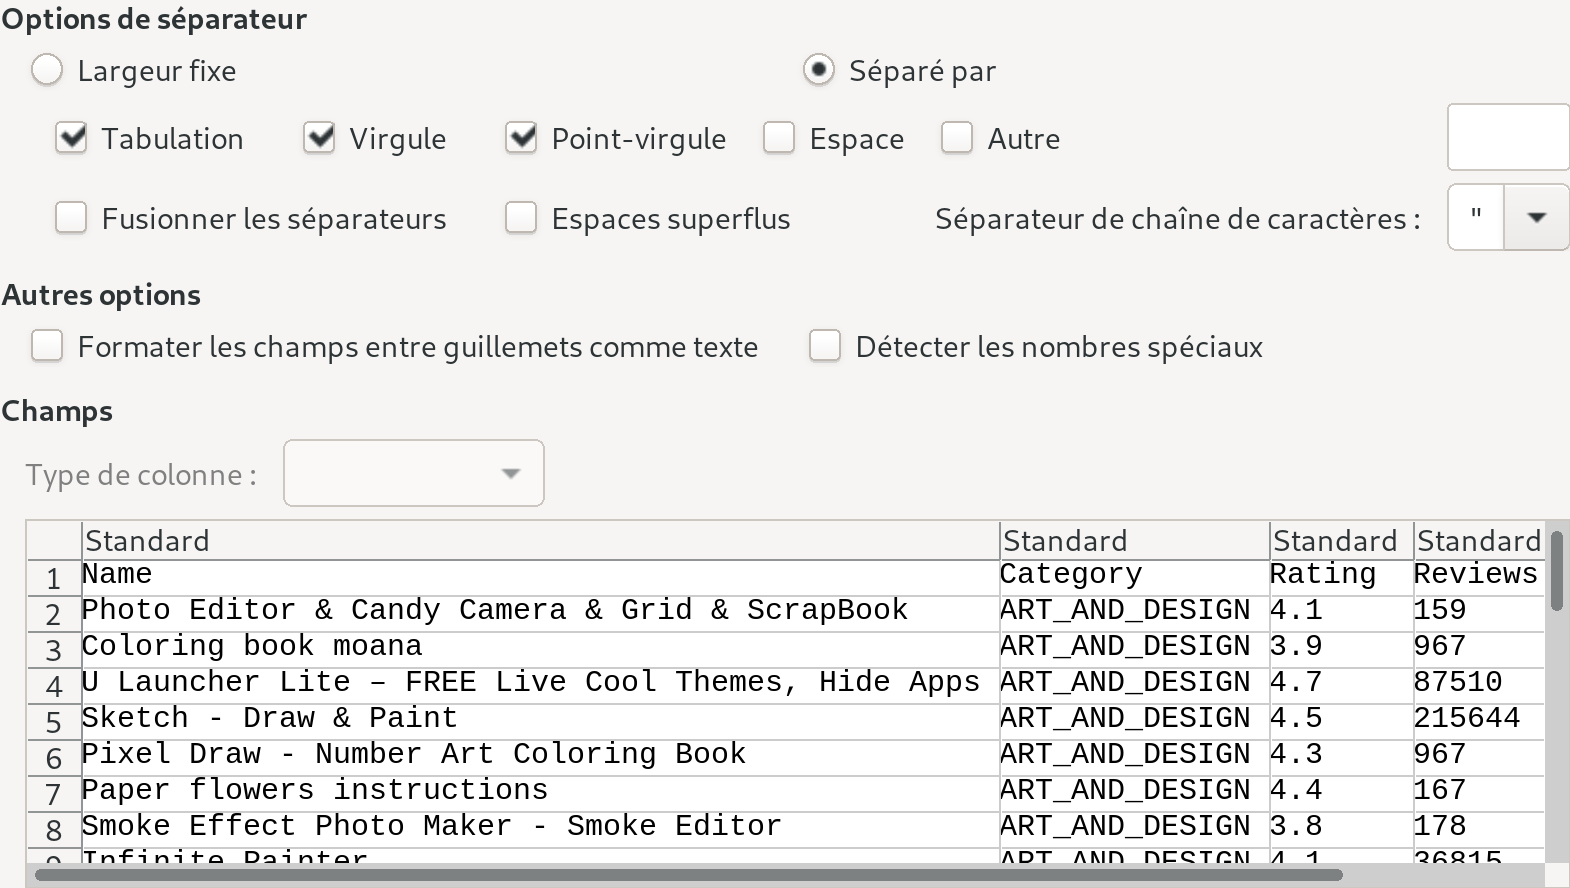
\includegraphics[width=8cm]{ressources/jeu-donnees.png}
        \captionof{figure}{Fichier csv ouvert avec LibreOffice}
        \label{IMG}
    \end{center}

\end{frame}
\begin{frame}
    \frametitle{csv (Comma Separated Values)}
    \begin{center}
        \begin{tabular}{|*{3}{c}|}
            \hline
            "Turing" ;     & "Alan" ;  & "19"   \\
            "Von Neuman" ; & "John";   & "18"   \\
            "Dijkstra"  ;  & "Edsger"; & "17.5" \\
            "Church"   ;   & "Alonso"; & "19"   \\
            \hline
        \end{tabular}
    \end{center}
    \begin{itemize}
        \item Chaque ligne représente un nouvel élément du jeu de données.
        \item Virgules, point-virgules ou tabulations.
        \item Attributs pas forcément présents.
        \item Guillemets pour encapsuler les données.
    \end{itemize}

    \note{Que se passe-t-il s'il y a des virgules dans une cellule? $\rightarrow$ guillemets}

\end{frame}
\begin{frame}
    \frametitle{}

    \begin{activite}
        \begin{enumerate}
            \item Télécharger et décompresser l'annexe \emph{googleplaystore.zip} sur le site \url{https://cviroulaud.github.io}
            \item Ouvrir le fichier \emph{googleplaystore.csv} avec un tableur (LibreOffice).
            \item Repérer les \emph{attributs}.
                  %traduire
        \end{enumerate}
    \end{activite}

\end{frame}
\begin{frame}
    \frametitle{Correction}

    \begin{itemize}
        \item \emph{Name:} nom,
        \item \emph{Category:} catégorie d'application,
        \item \emph{Rating:} note (sur 5),
        \item \emph{Reviews:} nombre de commentaires,
        \item \emph{Installs:} nombre d'installations.

    \end{itemize}

\end{frame}
\subsection{Lire un fichier \emph{csv}}
\begin{frame}[fragile]
    \frametitle{Lire un fichier externe avec Python}

    \begin{center}
        \begin{lstlisting}[language=Python]
# ouvrir le fichier
fichier = open("notes.csv")

# utiliser le fichier

# libérer le fichier
fichier.close()
    \end{lstlisting}
        \captionof{code}{Ouvrir et fermer}
        \label{iterer}
    \end{center}
\end{frame}

\begin{frame}[fragile]
    \frametitle{Lire un fichier externe avec Python}

    \begin{center}
        \begin{lstlisting}[language=Python]
import csv
# ouvrir le fichier
fichier = open("notes.csv")

lecteur = csv.reader(fichier)
for ligne in lecteur:
    print(ligne)

# libérer le fichier
fichier.close()
    \end{lstlisting}
        \captionof{code}{Méthode pour itérer sur les données}
        \label{iterer}
    \end{center}
    \note{Pour lire un fichier externe dans un programme Python, il faut d'abord ouvrir ce fichier à l'aide de la commande \textbf{\texttt{open}}. Ensuite la bibliothèque \texttt{csv} propose plusieurs méthodes pour itérer sur les lignes du fichier ouvert.}
\end{frame}

\begin{frame}
    \frametitle{}

    \begin{activite}
        \begin{enumerate}
            \item Tester le code \ref{iterer}.
            \item Remplacer la méthode \textbf{\texttt{reader}} par \textbf{\texttt{DictReader}}.
            \item Quel itérateur semble le plus adapté?
            \item Créer un programme \emph{appgoogle.py}.
            \item Dans le programme, ouvrir le fichier \emph{googleplaystore.csv}.
            \item Créer un tableau de dictionnaires à partir des données du fichier \emph{csv}.
        \end{enumerate}
    \end{activite}


\end{frame}
\begin{frame}[fragile]
    \frametitle{Correction}
    \lstinputlisting[firstline=12 ,lastline=14 ]{"scripts/lire-csv.py"}
    \begin{pycode}
import csv
fichier = open("scripts/notes.csv")

lecteur1 = csv.reader(fichier)
for ligne in lecteur1:
    print(ligne)
    print()

fichier.close()
    \end{pycode}

\end{frame}
\begin{frame}[fragile]
    \frametitle{Correction}
    \lstinputlisting[firstline=20 ,lastline=22 ]{"scripts/lire-csv.py"}
    \begin{pycode}
import csv
fichier = open("scripts/notes.csv")

lecteur1 = csv.DictReader(fichier)
for ligne in lecteur1:
    print(ligne)
    print()

fichier.close()
    \end{pycode}
\end{frame}
\begin{frame}
    \frametitle{Correction}

    \begin{itemize}
        \item On utilisera préférentiellement la méthode \textbf{\texttt{DictReader}}: chaque donnée est étiquetée.
        \item \texttt{\textbf{reader}} et \texttt{\textbf{DictReader}} sont des itérateurs: on ne peut les parcourir qu'une fois
    \end{itemize}

\end{frame}
\begin{frame}[fragile]
    \frametitle{Correction}

    \begin{aretenir}[Commentaire]
        Une variable de type \emph{OrderedDict} sera vue comme un simple dictionnaire.
    \end{aretenir}
    \begin{center}
        \begin{lstlisting}[language=Python, basicstyle=\small]
{"nom": "Turing", "prenom": "Alan", "moyennes": "19"}
{"nom": "Von Neuman", "prenom": "John", "moyennes": "18"}
{"nom": "Dijkstra", "prenom": "Edsger", "moyennes": "17.5"}
{"nom": "Church", "prenom": "Alonso", "moyennes": "19"}

\end{lstlisting}
        \captionof{code}{OrderedDict $\rightarrow$ dict}
        \label{CODE}
    \end{center}
\end{frame}

\begin{frame}[fragile]
    \frametitle{Correction}

    \begin{center}
        \begin{lstlisting}[language=Python]
import csv
# charge le fichier dans le programme
fichier = open("googleplaystore.csv")

# crée un itérateur sur les données
lecteur_donnees = csv.DictReader(fichier)

table = []
for ligne in lecteur_donnees:
    table.append(ligne)

# libère le fichier externe
fichier.close()
\end{lstlisting}
        \captionof{code}{Liste de OrderedDict}
        \label{CODE}
    \end{center}

\end{frame}

\begin{frame}[fragile]
    \frametitle{Correction}

    \begin{center}
        \begin{lstlisting}[language=Python]
import csv
# charge le fichier dans le programme
fichier = open("googleplaystore.csv")

# crée un itérateur sur les données
lecteur_donnees = csv.DictReader(fichier)

table = list(lecteur_donnees)

# libère le fichier externe
fichier.close()
\end{lstlisting}
        \captionof{code}{Liste de OrderedDict - seconde méthode}
        \label{CODE}
    \end{center}

\end{frame}

\begin{frame}[fragile]
    \frametitle{Correction}

    \begin{center}
        \begin{lstlisting}[language=Python, basicstyle=\small]
import csv
# charge le fichier dans le programme
fichier = open("googleplaystore.csv")
# crée un itérateur sur les données
lecteur_donnees = csv.DictReader(fichier)

table = []
# Pour chaque ligne
for ligne in lecteur_donnees:
    dico = {}
    # Pour chaque couple de la ligne
    for nom, val in ligne.items():
        dico[nom] = val
    table.append(dico)
# libère le fichier externe
fichier.close()
\end{lstlisting}
        \captionof{code}{liste de dictionnaires}
        \label{CODE}
    \end{center}

\end{frame}

\section{Manipuler les données}
\subsection{Valider les données}
\begin{frame}
    \frametitle{}
    Par défaut les données chargées dans un programme par la bibliothèque \textbf{\texttt{csv}} sont des chaînes de caractère.
    \begin{activite}
        Modifier le programme précédent pour typer correctement les informations récoltées.
    \end{activite}
    \note{note $\rightarrow$ flottants, Installs et Reviews $\rightarrow$entiers

        booléan possible aussi (payante/gratuite)
    }
\end{frame}

\begin{frame}[fragile]
    \frametitle{Correction}

    \begin{center}
        \begin{lstlisting}[language=Python, basicstyle=\small, xleftmargin=1em, xrightmargin=1em]
table = []
for ligne in lecteur_donnees:
    dico = {}
    for nom, val in ligne.items():
        # validation des données
        if nom == "Rating":
            val = float(val)
        if nom == "Installs" or nom == "Reviews":
            val = int(val)

        dico[nom] = val
    table.append(dico)
\end{lstlisting}
        \captionof{code}{Tentative de conversion des données}
        \label{CODE}
    \end{center}

    \colorbox{LightCoral}{ValueError: invalid literal for int() with base 10: 'NaN'
    }
\end{frame}
\begin{frame}
    \frametitle{Correction}

    \begin{center}
        \begin{tabular}{|*{5}{c|}}
            \hline
            Name       & Category & Rating & Reviews & Installs \\
            \hline
            CX Network & BUSINESS & NaN    & 0       & NaN      \\
            \hline
        \end{tabular}
        \captionof{table}{Des valeurs particulières}
    \end{center}
    \note[item]{Installs: NaN $\rightarrow$0}
    \note[item]{Rating: NaN $\rightarrow$ -1 (pas notée)}
\end{frame}
\begin{frame}[fragile]
    \frametitle{Correction}
    \begin{center}
        \begin{lstlisting}[language=Python, basicstyle=\small, xleftmargin=1em, xrightmargin=1em]
table = []
for ligne in lecteur_donnees:
    dico = {}
    for nom, val in ligne.items():
        if nom == "Rating":
            if val == "NaN":
                val = -1.0
            else:
                val = float(val)
        if nom == "Installs":
            if val == "NaN":
                val = 0
            else:
                val = int(val)
        dico[nom] = val
    table.append(dico)
\end{lstlisting}
        \captionof{code}{Conversion des données}
        \label{CODE}
    \end{center}
    \note{non noté = -1}
\end{frame}
\subsection{Rechercher des données}
\begin{frame}
    \frametitle{Imiter un moteur de recherche}

    Une action courante sur un jeu de données est de sélectionner certaines lignes en fonction d'un critère.

\end{frame}

\subsubsection{Sélectionner}
\begin{frame}
    \frametitle{}

    \begin{activite}
        \begin{enumerate}
            \item Écrire la fonction \textbf{\texttt{trouver\_app(mot\_cle: str, tab: list) $\rightarrow$ list}} qui renvoie la liste des applications du tableau \emph{tab} dont le nom contient \emph{mot\_cle}.\\
                  \underline{Indication:} L'instruction \textbf{\texttt{in}} permet de vérifier si une sous-chaîne est présente dans une chaîne de caractère.
                  %tous les mots commencent par une majuscule
            \item Chercher toutes les applications dont le nom contient le mot \emph{Photo}.
            \item Compter le nombre d'applications renvoyées.
        \end{enumerate}
    \end{activite}

\end{frame}
\begin{frame}
    \frametitle{Correction}

    \lstinputlisting[firstline=12 ,lastline=22, basicstyle=\small, xrightmargin=1em ]{"scripts/appgoogle.py"}

\end{frame}
\begin{frame}[fragile]
    \frametitle{Correction}

    \begin{center}
        \begin{lstlisting}[language=Python, basicstyle=\small]
applications = trouver_app("Photo", table)
len(applications)
\end{lstlisting}
    \end{center}
\end{frame}

\begin{frame}
    \frametitle{}
    \setcounter{compteuractivite}{3}
    \begin{activite}
        \begin{enumerate}
            \setcounter{enumi}{3}

            \item Écrire la fonction \textbf{\texttt{meilleur\_app\_notee(tab: list) $\rightarrow$ dict}} qui renvoie l'application la mieux notée du tableau \emph{tab}.
            \item Trouver l'application photo la mieux notée.
            \item \underline{Pour les plus avancés:} en s'aidant de la documentation, modifier la fonction \textbf{\texttt{trouver\_app}} pour quelle:
                  \begin{itemize}
                      \item ne prenne pas en compte la casse des mots,
                      \item renvoie les applications contenant plusieurs mots-clés; les mots sont passés à la fonction par le paramètre \emph{mot\_cle} séparés par un espace.
                  \end{itemize}
        \end{enumerate}
    \end{activite}

\end{frame}
\begin{frame}[fragile]
    \frametitle{Correction}

    \lstinputlisting[firstline=42 ,lastline=52, basicstyle=\small ]{"scripts/appgoogle.py"}
    \begin{center}
        \begin{lstlisting}[language=Python, basicstyle=\small]
applications = trouver_app("Photo", table)
meilleur_app_notee(applications)
\end{lstlisting}
    \end{center}

\end{frame}
\subsubsection{Agréger}
\begin{frame}
    \frametitle{Agréger des données}

    On peut imaginer proposer à l'utilisateur toutes les applications notées au-dessus de la moyenne.
    \begin{activite}
        \begin{enumerate}
            \item Écrire la fonction \textbf{\texttt{moyenne\_note(tab: list)  $\rightarrow$ float}} qui calcule la note moyenne des applications de \emph{tab}. Le résultat sera arrondi à deux chiffres significatifs.
            \item Dans le programme principal, construire \emph{par compréhension }le tableau des applications photo dont la note est strictement supérieure à la moyenne.
        \end{enumerate}
    \end{activite}
    \note{
        La sélection précédente étant très restrictive, il peut être intéressant d'offrir un choix plus large. }
\end{frame}
\begin{frame}
    \frametitle{Correction}

    \lstinputlisting[firstline=55 ,lastline=66, basicstyle=\small ]{"scripts/appgoogle.py"}

\end{frame}
\begin{frame}[fragile]
    \frametitle{Correction}

    \begin{center}
        \begin{lstlisting}[language=Python, basicstyle=\small]
applications = trouver_app("Photo", table)

moyenne = moyenne_note(applications)

meilleur_app = [app for app in applications if app["Rating"] > moyenne]
\end{lstlisting}
        \captionof{code}{Sélection par compréhension}
        \label{CODE}
    \end{center}

\end{frame}
\subsection{Trier des données}
\begin{frame}
    \frametitle{Trier}

    Le tri est une autre opération fréquemment exécutée sur un jeu de données. On peut imaginer dans notre cas, ordonner les applications photo en fonction de leur note.

\end{frame}

\subsubsection{Tri natif}
\begin{frame}[fragile]
    \frametitle{}

    En tant que langage de haut-niveau Python offre un outil de tri efficace:
    \begin{itemize}
        \item la méthode \textbf{\texttt{sort}} trie \emph{en place} un itérable,
              \begin{center}
                  \begin{lstlisting}[language=Python]
ma_liste.sort()
    \end{lstlisting}
              \end{center}
        \item la fonction \textbf{\texttt{sorted}} crée un nouvel itérable trié.
              \begin{center}
                  \begin{lstlisting}[language=Python]
nouvelle = sorted(ma_liste)   
    \end{lstlisting}
              \end{center}
    \end{itemize}

\end{frame}

\subsubsection{Clé de tri}
\begin{frame}[fragile]
    \frametitle{}

    Dans notre cas les objets triés ne sont pas des simples entiers mais des dictionnaires. Il faut alors préciser la \textbf{clé de tri}.
    \lstinputlisting[firstline=21 ,lastline=27, basicstyle=\small]{"scripts/tri-cle.py"}
\note{Certains élèves ont la même note $\rightarrow$second critère?}
\begin{pycode}
import csv

f = open("scripts/notes.csv")
data = csv.DictReader(f)
eleves = []
for e in data:
    dico = {"nom": e["nom"], "prenom": e["prenom"],
            "moyennes": float(e["moyennes"])}
    eleves.append(dico)
f.close()


def parametres_tri(eleve: dict) -> float:
    """
    renvoie le paramètre utilisé pour le tri
    """
    return eleve["moyennes"]

eleves.sort(key=parametres_tri)
for e in eleves:
    print(e)
    print()
    \end{pycode}
\end{frame}

\begin{frame}
    \frametitle{}

    \begin{activite}
        \begin{enumerate}
            \item Écrire la fonction \textbf{\texttt{parametres\_tri\_1(app: dict) $\rightarrow$ float}} qui renvoie la note de l'application.
            \item Trier le tableau des applications photo en fonction de leur note.
            \item Afficher les cinq meilleures applications.
        \end{enumerate}
    \end{activite}

\end{frame}
\begin{frame}
    \frametitle{Correction}

\lstinputlisting[firstline=69 ,lastline=73, basicstyle=\small, xleftmargin=1em, xrightmargin=1em ]{"scripts/appgoogle.py"}


\end{frame}
\begin{frame}[fragile]
    \frametitle{Correction}
    \lstinputlisting[firstline=135 ,lastline=137, basicstyle=\small, xleftmargin=1em, xrightmargin=1em ]{"scripts/appgoogle.py"}
\begin{center}
\begin{lstlisting}[language=bash]
Top 1: Simple Photo BG Changer
Top 2: FG Autumn Photo Puzzle
Top 3: Blender BG - Photo Blend With Background
Top 4: Best CG Photography
Top 5: Life Made WI-Fi Touchscreen Photo Frame 
\end{lstlisting}
\end{center}

\end{frame}
\begin{frame}
    \frametitle{}
\setcounter{compteuractivite}{5}
    \begin{activite}
        Pour départager les applications avec la même note, on choisit de définir un second paramètre de tri: le nombre de commentaires.
        \begin{enumerate}
            \setcounter{enumi}{3}
            \item Écrire la fonction \textbf{\texttt{parametres\_tri\_2(app: dict) $\rightarrow$ tuple}} nouvelle clé de tri.
            \item Appliquer cette nouvelle clé.
        \end{enumerate}
    \end{activite}

\end{frame}
\begin{frame}[fragile]
    \frametitle{Correction}

\lstinputlisting[firstline=76 ,lastline=80, basicstyle=\small, xleftmargin=1em, xrightmargin=1em ]{"scripts/appgoogle.py"}
\begin{center}
    \begin{lstlisting}[language=bash]
Top 1: FG Autumn Photo Puzzle
Top 2: Blender BG - Photo Blend With Background
Top 3: Simple Photo BG Changer
Top 4: Best CG Photography
Top 5: Life Made WI-Fi Touchscreen Photo Frame
    \end{lstlisting}
    \end{center}


\end{frame}

\begin{frame}
    \frametitle{}
\setcounter{compteuractivite}{5}
    \begin{activite}
        \begin{enumerate}
            \setcounter{enumi}{5}
            \item \underline{Pour les plus avancés:} Reprendre la fonction \textbf{\texttt{tri\_insertion}} et la modifier pour effectuer le tri de la première question.
        \end{enumerate}
    \end{activite}

\end{frame}
\begin{frame}
    \frametitle{Correction}

    \lstinputlisting[firstline=83 ,lastline=96, basicstyle=\small, xleftmargin=1em, xrightmargin=1em ]{"scripts/appgoogle.py"}

\end{frame}
\end{document}